\chapter{The Search for Invisible Decays of the Higgs Boson}
\label{sec:vbf}

The discovery of the SM Higgs boson~\needcite~involved multiple production modes.
Gluon fusion has the largest cross section (49 pb) at the LHC because of the large gluon PDF, followed by vector boson fusion (VBF) (3.8 pb), $WH$ (1.4 pb), and $ZH$ (0.89 pb)~\cite{lhchxswg}.
While gluon fusion is the most frequent mode, the unique detector signatures of the other production modes can be combined the various Higgs decay signatures to define a signal topology with few backgrounds.

Many DM models~\needcite~allow for DM fermions or scalars to acquire mass through the Higgs mechanism, coupling to the SM Higgs boson.
If the DM candidate $\chi$ satisfies $2m_\chi < m_H$, then we expect to observe $H\rightarrow\chi\bar\chi$.
From measurements of the visible branching fractions, we can indirectly place an upper bound of $\mathcal{B}(H\rightarrow\chi\bar\chi)<0.2$~\needcite.
In this chapter, we describe a direct search for $H\rightarrow\chi\bar\chi$ decays.

As with the case of the mono-top search, the $H\rightarrow\chi\bar\chi$ process manifests as \ptmiss. 
Each of the aforementioned Higgs production modes translates into a $\ptmiss+X$ signature, where $X$ refers to one or more SM particles.
Figure~\ref{fig:vbf:hdiags} shows each of the signatures; in this chapter, we will focus on the VBF production mode, as the unique final state topology provides the best sensitivity to $H\rightarrow\chi\bar\chi$.

\begin{figure}
    \begin{center}
        \begin{subfigure}[t]{0.32\textwidth}
            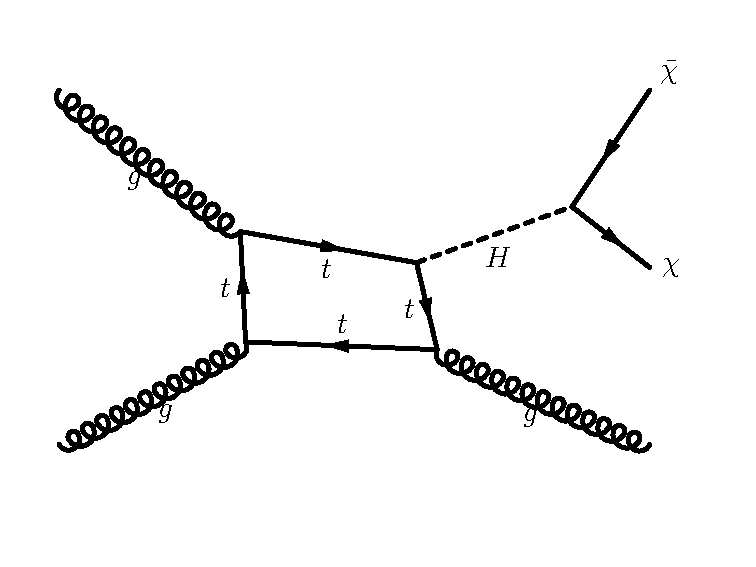
\includegraphics[width=\textwidth]{figures/vbf/diagrams/ggf_hinv.pdf}
            \caption{$gg\rightarrow H(\rightarrow\chi\bar\chi)$+jet(s)}
        \end{subfigure}
        \begin{subfigure}[t]{0.32\textwidth}
            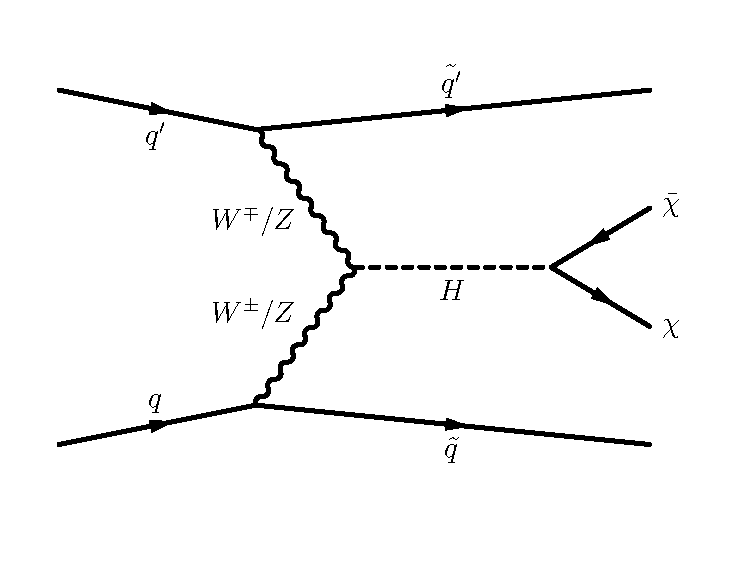
\includegraphics[width=\textwidth]{figures/vbf/diagrams/vbf_hinv.pdf}
            \caption{$qq'\rightarrow H(\rightarrow\chi\bar\chi)$+jet(s)}
        \end{subfigure}
        \begin{subfigure}[t]{0.32\textwidth}
            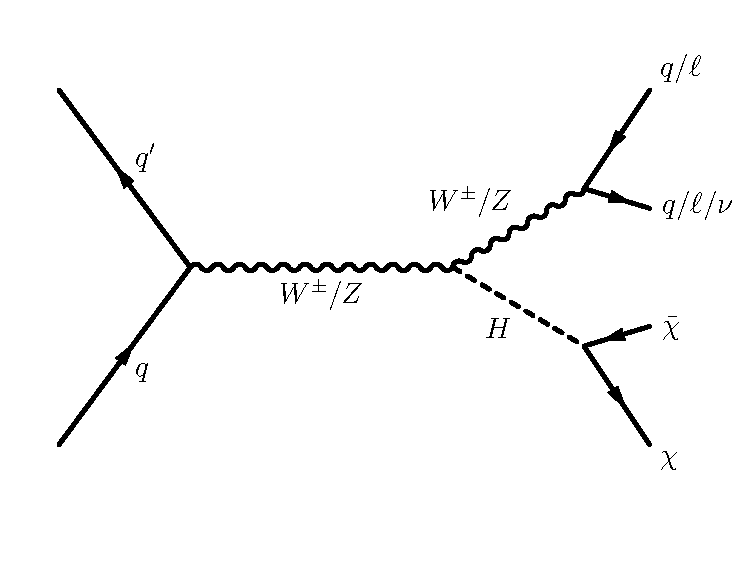
\includegraphics[width=\textwidth]{figures/vbf/diagrams/zh_hinv.pdf}
            \caption{$qq'\rightarrow VH(\rightarrow\chi\bar\chi)$}
        \end{subfigure}
        \caption{Diagrams that contribute to the production of the SM Higgs boson at the LHC, with the subsequent decay to DM candidates.
                 The shown diagrams are all chosen to generate large $\ptmiss$ through the presence of one or more SM particles in the final state.}
        \label{fig:vbf:hdiags}
    \end{center}
\end{figure}

\section{Signal selection}

VBF $\hinv$ events are characterized by large $\ptmiss$ and two jets.
These jets are typically:
\begin{itemize}
    \item Fairly forward in the detector
    \item Far apart from each other in $\eta$
    \item Highly energetic (large $E$, moderate $\pt$)
    \item Close together in $\phi$
\end{itemize}
A candidate VBF $\hinv$ event displaying these properties is shown in a CMS event display in Figure~\ref{fig:vbf:ed}.

\begin{figure}[]
    \begin{center}
        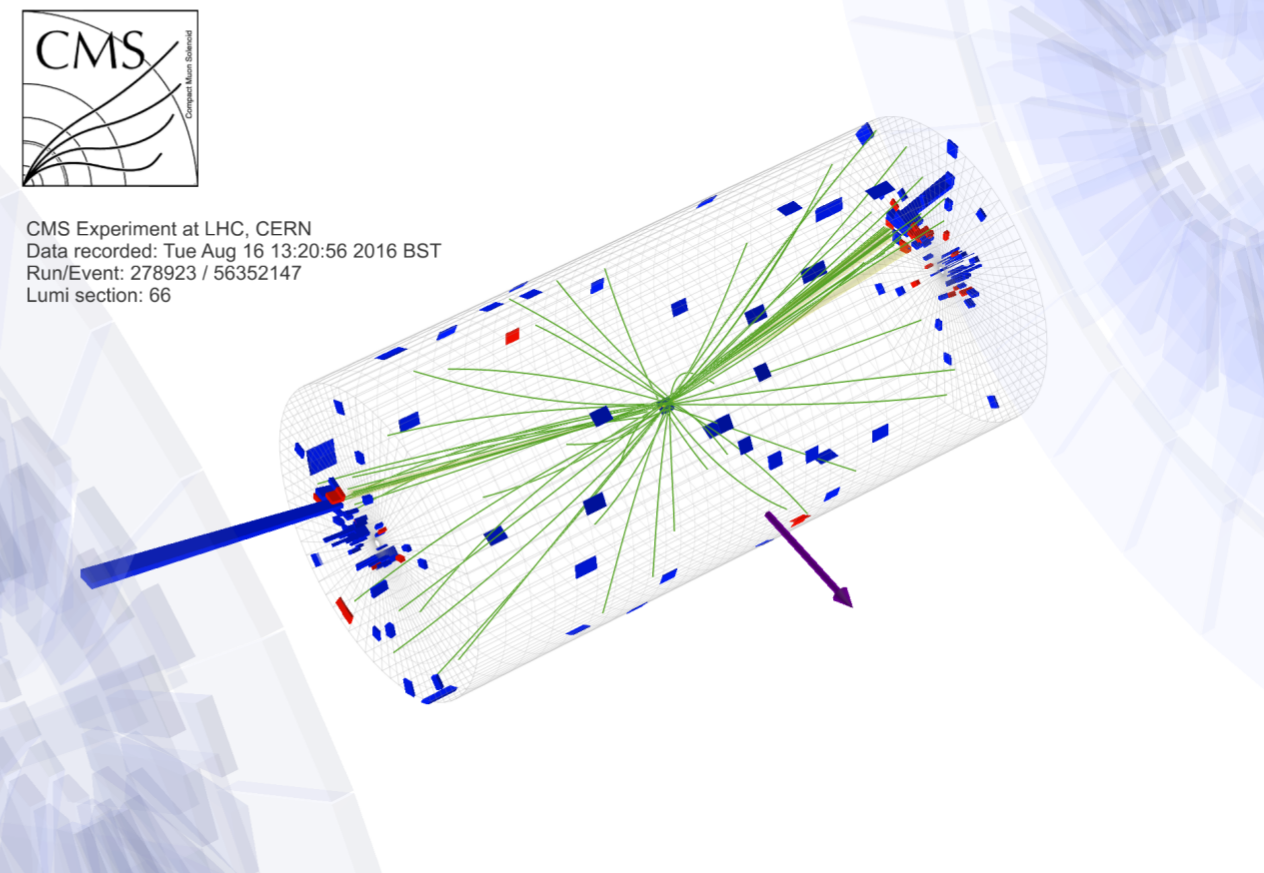
\includegraphics[width=0.8\textwidth]{figures/vbf/misc/event_display.png}
        \caption{Candidate VBF $\hinv$ event with two energetic forward jets ($\pt=180,~107$ GeV) and large $\ptmiss$ ($360$ GeV).
                 Red (blue) towers represent deposits in the hadronic (electromagnetic) calorimeter.
                 Green lines are tracks reconstructed from hits of charged particles in the tracker. 
                 The blue arrow represents the direction and magnitude of the $\ptmiss$.}
        \label{fig:vbf:ed}
    \end{center}
\end{figure}

\subsection{Online trigger selection}

The same trigger decisions (L1 and HLT) as described in Section~\ref{sec:mt:trigger} are used to select events in this analysis.
However, the L1 seeds for the 2016 data run were designed with mono-top-like analyses in mind; i.e., searches where the momentum imbalance is created by central objects.
To avoid noise and resolution issues in the forward calorimeters, the L1 seed only considers energy deposits in the region $|\eta|<3$. 
Therefore, VBF events in which both jets are in the forward region will not be triggered.  

\subsection{EW and QCD production of electroweak bosons}

\subsection{Sensitivity optimization}

\section{Background estimation}

\section{Results}

\subsection{Constraints on Higgs production and decay parameters}

\subsection{Constraints on scalar production of DM}

